Given $K$ the number of drones and
$N, M$ the grid sizes, the number of rows, and the number of columns, respectively. We can analyze our algorithm regarding these inputs using asymptotic computational complexity.

The complexity of our algorithm is the worst case of a BFS in the temporal graph, considering the $\mathcal{O}(\log S)$ from the scheduled structure, where $S= N M T$ is the size of the search space. It can be seen that this would be $\mathcal{O}(N M T)\mathcal{O}(\log N M T)$, where $T$ is the maximum time a drone lands. However, $T$ is surely bounded by $\mathcal{O}(K N M)$. In addition, it can be shown that $T$ is bounded by $\mathcal{O}((N+M) K)$. An intuitive view of this is shown in \ref{fig:worst_path}, where we have three drones on a $3\times 4$ grid with the same initial position($s_i$) and final position($g_i$), where $i=1\dots3$. In this case, the shorter path for each drone is $n+m$,$n=3;m=4$, and in the worst case, we will wait for each drone to complete its path, thus $k(n+m)$ is an upper bound for our heuristic since our heuristic always chooses a shorter path than $k(n+m)$ because we do not wait for each drone to complete the path.   Then the complexity is bounded by $$\mathcal{O}((N+M) K N M \log((N+M) K N M))= \mathcal{O}(\max{(N,M)} N M K  \log(\max{(N,M)} N M K)) $$  $\approx \mathcal{O}(N^3  K \log(N^3 K) = \mathcal{O}(N^3  K \max{(\log N , \log K))} $, if the grid is square. 



\begin{figure}[H]
    \centering
    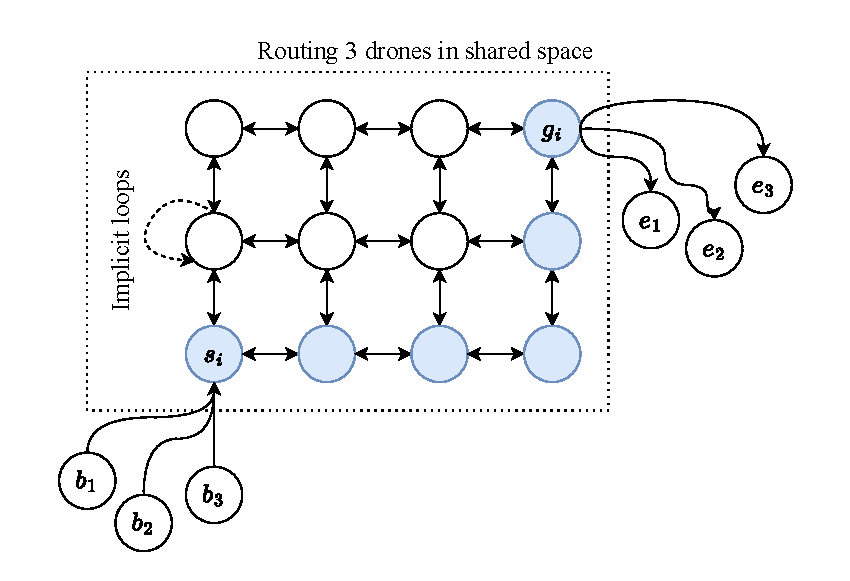
\includegraphics[width=0.8\textwidth]{img/worst_path.drawio.pdf}
    \caption{Worst case path.}
    \label{fig:worst_path}
\end{figure}
